In diesem Kapitel wird die technische Realisierung des Gamification-Konzepts detailliert beschrieben. Die Umsetzung erfolgte in zwei getrennten Codebasen: einer PHP-basierten API 
im Backend sowie einer mobilen Applikation auf Basis von Vue.js und TypeScript.

\subsection{Erweiterung der Backend-Infrastruktur (API)}

Ein zentraler Aspekt der technischen Umsetzung war die Erweiterung des bestehenden Datenmodells, um die komplexen Anforderungen des Gamification-Konzepts abzubilden. Ziel der 
Architektur war eine strikte Trennung zwischen Datenhaltung und Präsentation (Separation of Concerns). Während die Applikation die Logik zum Rendern der Spielwelt enthält, 
werden sämtliche inhaltlichen und strukturellen Informationen dynamisch über die API bezogen. Dies ermöglicht es, neue Lerninhalte zu pflegen, ohne ein Update der App-Software
 durchführen zu müssen.

\begin{figure}[htbp]
    \centering
    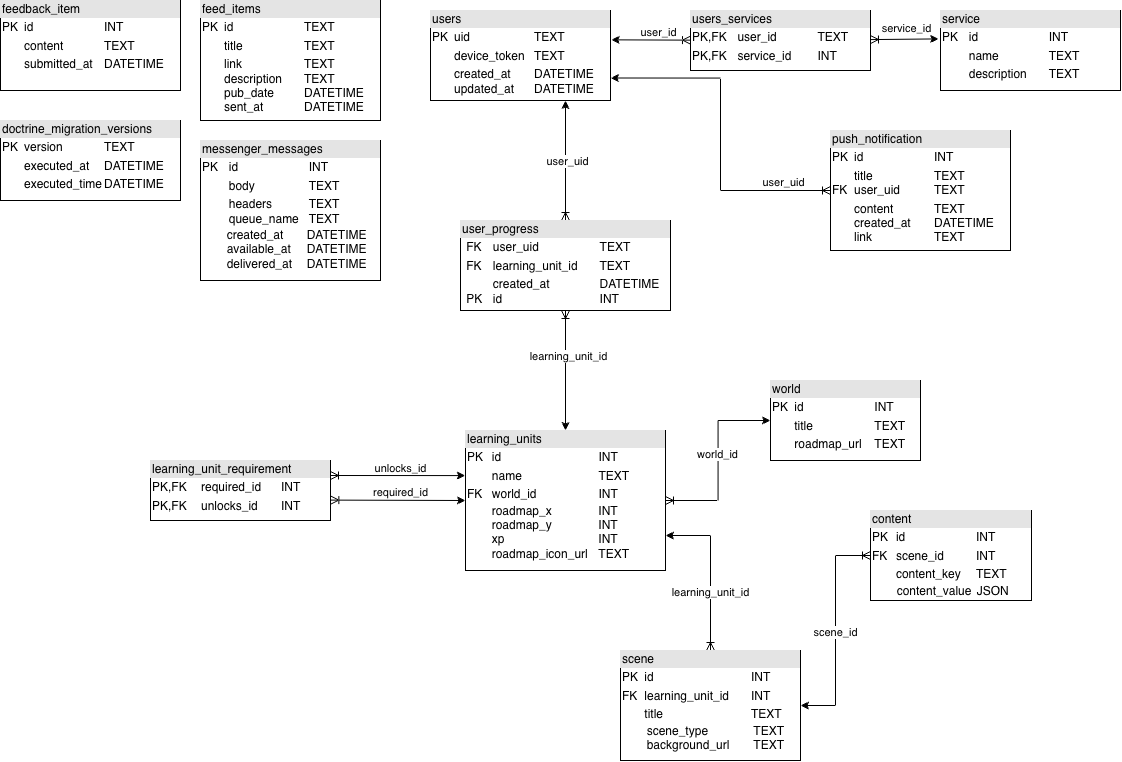
\includegraphics[width=0.9\textwidth]{figures/ER-Schema.png}
    \caption{ER-Schema der GameUp-Datenbank}
    \label{fig:er_schema}
\end{figure}

Um die Anforderungen der TU München technisch umzusetzen, wurden sechs zentrale Tabellen in das bestehende Schema integriert (siehe Abbildung \ref{fig:er_schema}):

\begin{itemize}
    \item \textbf{world \& scene:} Diese Tabellen bilden die topografische Hierarchie ab. Analog zu Videospiel-Klassikern wie „Super Mario Bros.“ ist das System auf Skalierbarkeit 
    ausgelegt: Eine Welt fungiert als Container für thematisch zusammenhängende Szenen (z. B. „Lissabon“ oder „Cyber-City“), die wiederum den narrativen Rahmen für die Lerninhalte 
    vorgeben.
    \item \textbf{learning\_units:} Hier werden die eigentlichen didaktischen Einheiten verwaltet. Durch die Verknüpfung mit Szenen signalisiert die API der App, welche Lerninhalte 
    an welchem Ort der grafischen Spielwelt aktiv sind.
    \item \textbf{learning\_unit\_requirement:} Zur Steuerung des Lernpfads wurde eine Abhängigkeitslogik implementiert. Diese Tabelle definiert Voraussetzungen (Prerequisites), sodass 
    bestimmte Einheiten erst nach dem erfolgreichen Abschluss vorangegangener Aufgaben freigeschaltet werden.
    \item \textbf{content:} Um eine maximale Flexibilität zu gewährleisten, wurde die Content-Tabelle hochgradig abstrakt entworfen. Sie speichert unterschiedliche Datentypen. Von URLs 
    für Bild-Assets der Comic-Szenen bis hin zu JSON-strukturierten Inhalten für Formulare. Die App fungiert hierbei lediglich als „Renderer“, der die Daten gemäß 
    ihrem Typ interpretiert.
    \item \textbf{user\_progress:} Diese Tabelle persisitiert den individuellen Fortschritt der Nutzer. Sie bildet die Grundlage für das serverseitige Belohnungssystem und stellt sicher,
     dass der Spielstatus geräteübergreifend synchron bleibt.
\end{itemize}

Die technische Realisierung dieser Struktur erfolgte mit PHP und dem Symfony-Framework. Durch den Einsatz von Doctrine ORM konnten die Relationen zwischen Welten, Anforderungen und 
Fortschritten typsicher abgebildet werden. Auf Basis des aktualisierten Schemas wurden die Framework-typischen Komponenten, insbesondere Repositories für den Datenbankzugriff, 
Service-Klassen für die Business-Logik und REST-Controller für die Bereitstellung der Endpunkte, entwickelt.

Ein wesentlicher Bestandteil der API-Architektur ist das Sicherheits- und Authentifizierungskonzept. Die gesamte Benutzerverwaltung sowie der Login-Mechanismus werden über 
\textbf{Firebase} realisiert. Zur Absicherung der Kommunikation wird bei jedem API-Aufruf ein von Firebase generierter User-Token im Header mitgeschickt. Dieser wird serverseitig 
validiert, um sicherzustellen, dass nur authentifizierte Nutzer Zugriff auf ihre Fortschrittsdaten haben. Die Abbildung \ref{fig:runtime_login} verdeutlicht diesen Prozess sowie 
die Interaktion zwischen der App, dem Identity Service und den externen Firebase-Schnittstellen während des Anmeldevorgangs.

\begin{figure}[htbp]
    \centering
    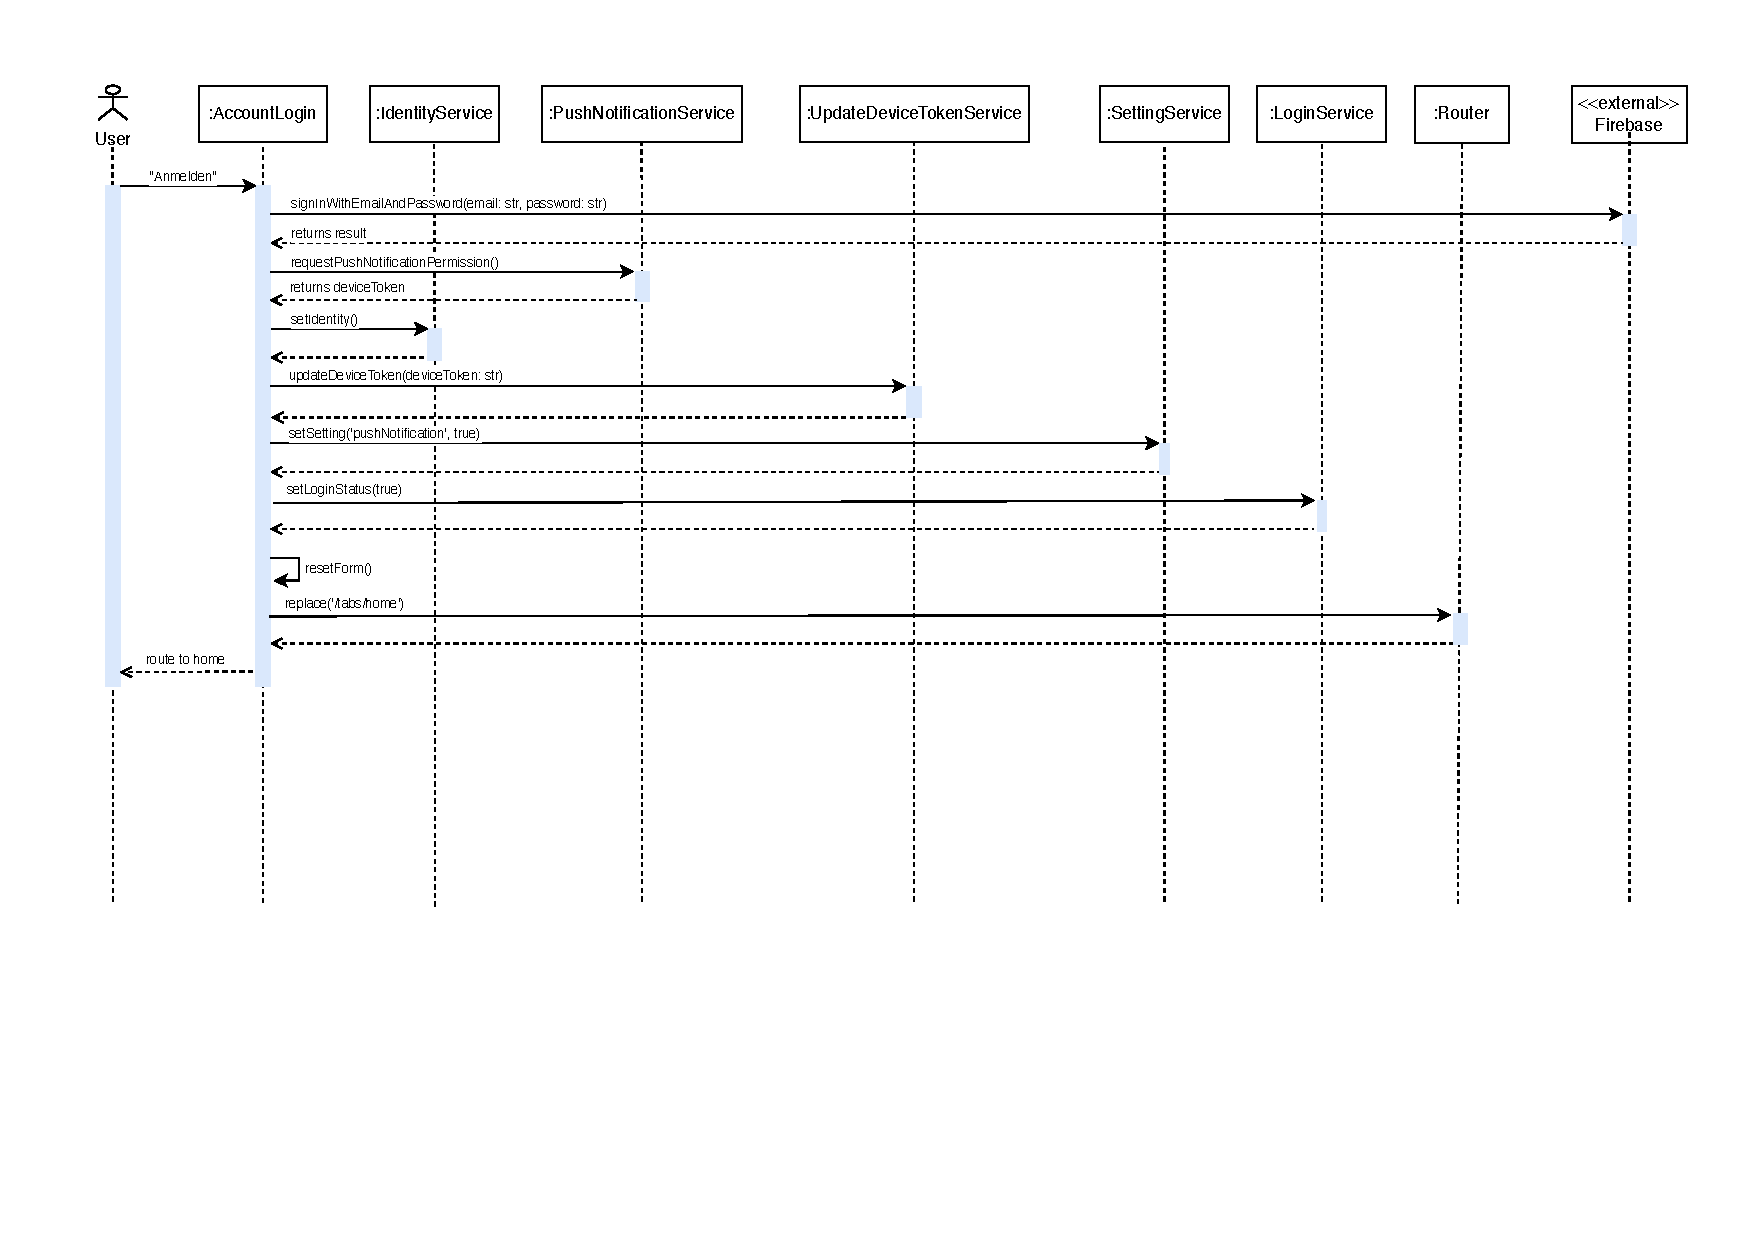
\includegraphics[width=0.8\textwidth]{figures/RuntimeDiagramLogin.pdf}
    \caption{Runtime-Diagramm des Authentifizierungsprozesses via Firebase}
    \label{fig:runtime_login}
\end{figure}

Durch diese Architektur erfolgt die Validierung der Freischalt-Logik (z. B. die Prüfung der Voraussetzungen aus der Tabelle \texttt{learning\_unit\_requirement}) ausschließlich 
serverseitig. Dies verhindert Manipulationen am Lernfortschritt effektiv, da die App lediglich die validierten Ergebnisse der API visualisiert, während die Hoheit über den tatsächlichen 
Status („Single Source of Truth“) im Backend verbleibt.

\subsection{Integration der Gamification-Schnittstellen in der App}

Nach der Bereitstellung der Datenstrukturen im Backend erfolgte die clientseitige Integration in die mobile Applikation. Diese basiert technologisch auf dem Framework 
\textbf{Vue.js} in Kombination mit dem Build-Tool \textbf{Vite}. Um eine hohe Typsicherheit und Wartbarkeit innerhalb der heterogenen Datenstrukturen des Projekts zu gewährleisten, 
wurde die gesamte Geschäftslogik konsequent in \textbf{TypeScript} umgesetzt.

\subsubsection{Datenmodellierung und Service-Layer}
Die Repräsentation der Backend-Entitäten erfolgt in der App über TypeScript-Interfaces (z. B. \texttt{ILearningUnit}). Diese dienen als Kontrakte für die Datenstrukturen und stellen 
sicher, dass die über die API bezogenen Objekte systemweit korrekt verwendet werden. Die Kommunikation mit dem Backend wurde durch dedizierte Service-Klassen gekapselt, welche die 
asynchronen Netzwerkanfragen über eine zentrale \texttt{BaseRequest}-Komponente abwickeln.

Ein wesentliches Merkmal dieser Architektur ist das automatisierte Mapping der API-Antworten in die entsprechenden Modelle. Wie das folgende Beispiel des \texttt{LearningUnitsService} 
zeigt, werden die Rohdaten (\texttt{any}) unmittelbar nach dem Empfang durch spezialisierte Mapping-Methoden transformiert:

\begin{verbatim}
static mapResponseToLearningUnit(raw: any[]): ILearningUnit[] {
    if (!Array.isArray(raw)) raw = [raw];

    return raw.map((item: any): ILearningUnit => ({
        id: item.id,
        name: item.name,
        xp: item.xp,
        unlocked: item.unlocked,
        completed: item.completed,
        scenes: item.scenes 
            ? SceneService.mapResponseToScene(item.scenes) 
            : [],
        world: item.world 
            ? WorldService.mapResponseToWorld(item.world)[0] 
            : undefined,
    }));
}
\end{verbatim}

\subsubsection{Abbildung der Gamification-Logik}
Der Service implementiert zudem die komplexen Filter- und Statuslogiken, die für die Visualisierung des Spielfortschritts notwendig sind. Durch spezialisierte Methoden wie 
\texttt{loadAll\-Unlocked\-Learning\-Units} oder \texttt{loadAllLockedLearningUnits} kann die App gezielt steuern, welche Inhalte dem Nutzer auf der Roadmap angezeigt werden. 

Besonderes Augenmerk wurde auf die Auflösung der Abhängigkeiten gelegt. Die Methode \texttt{mapRequirements} transformiert die relationalen Verknüpfungen aus der Datenbank 
(z. B. welche Einheit welche andere freischaltet) in einfache Arrays von Identifikatoren. Dies entlastet die UI-Komponenten von komplexen Logikoperationen und ermöglicht eine 
performante Prüfung des Freischaltstatus innerhalb der App-Oberfläche. Durch die Einbindung der \textbf{EndpointGroups} wird zudem sichergestellt, dass die API nur die für den 
jeweiligen Kontext notwendigen Datenfelder liefert, was die Netzwerklast minimiert und die Performance der mobilen Anwendung optimiert.

\subsection{Entwicklung einer leichtgewichtigen Game-Engine}

Um das Gamification-Konzept der TU München performant umzusetzen, wurde eine eigene Game-Engine auf Basis von TypeScript und dem HTML5-Canvas-API entwickelt. Die Architektur ist 
darauf ausgelegt, die von der API gelieferten Daten dynamisch zu interpretieren und in eine interaktive Abfolge von Szenen zu übersetzen.

\subsubsection{Der Engine-Core: Steuerung und Szenen-Management}
Das Fundament der Engine bildet der „Core“, der für den zentralen Rendering-Loop und das Management der Spielzustände verantwortlich ist. Die Steuerung erfolgt über die zentrale
 \texttt{Game}-Klasse. Ein wesentliches Merkmal ist das flexible Szenen-Management: Die Engine fungiert als Zustandsautomat, der zwischen verschiedenen Szenentypen wechselt.

\begin{figure}[htbp]
    \centering
    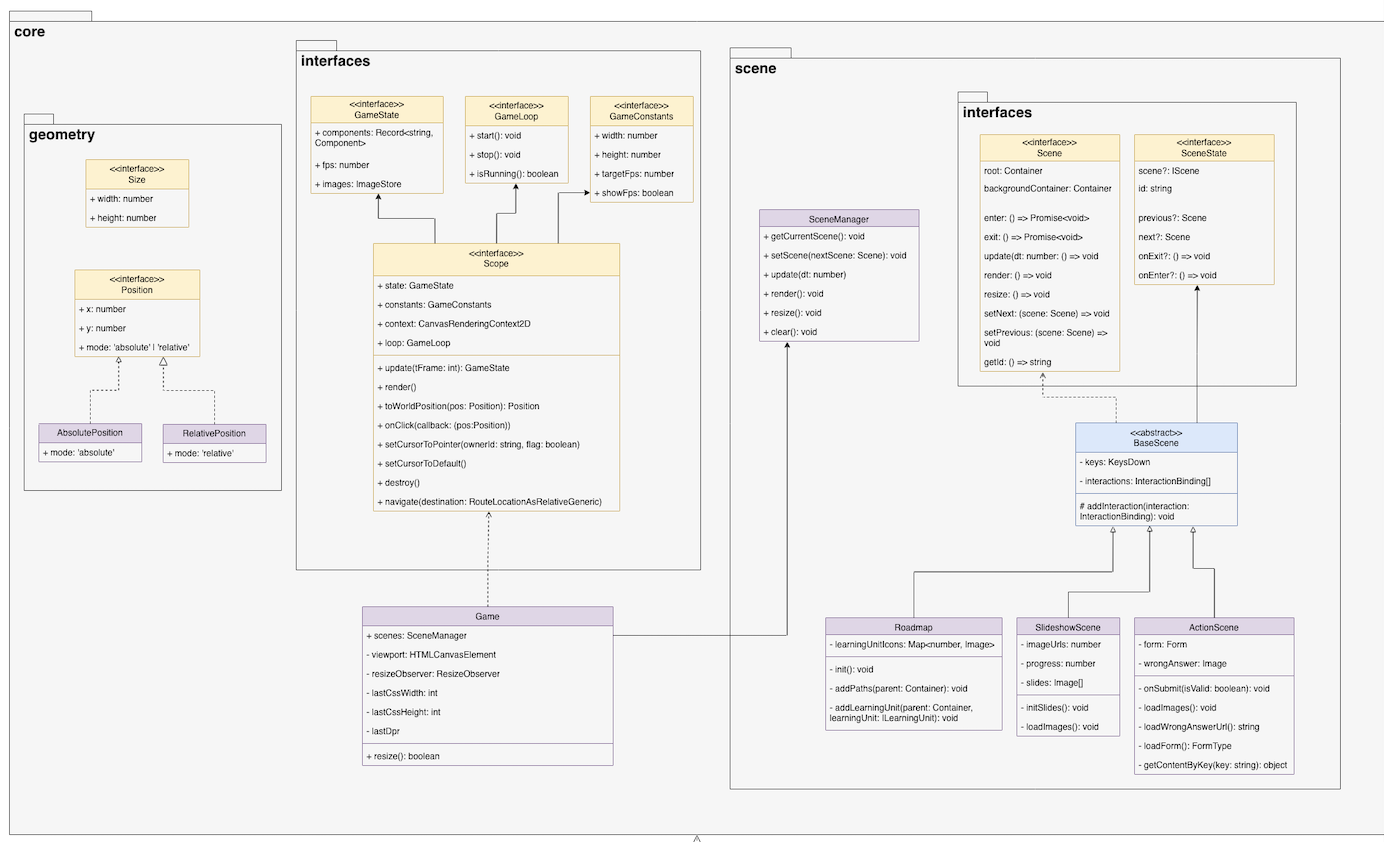
\includegraphics[width=0.85\textwidth]{figures/ClassDiagram_Core.png}
    \caption{Core-Architektur der Engine mit Fokus auf das Szenen-Management}
    \label{fig:engine_core}
\end{figure}

Die Integration in die App erfolgt über Vue-Komponenten wie die \texttt{LearningUnitView}. Beim Betreten der Ansicht (\texttt{onIonViewDidEnter}) wird die entsprechende Lerneinheit 
via API geladen und die Engine initialisiert. Eine \texttt{LearningUnit} folgt dabei einer festen didaktischen Struktur, die im Konzept der TU München definiert wurde:

\begin{itemize}
    \item \textbf{Opening:} Einstieg in die Thematik.
    \item \textbf{Problem:} Visualisierung der Risiken.
    \item \textbf{Learning:} Vermittlung von Fachwissen durch Learning Nuggets.
    \item \textbf{Action:} Durchführung einer interaktiven Challenge.
    \item \textbf{Reward:} Abschluss und Belohnung.
\end{itemize}

Diese Phasen werden durch die Engine als verkettete Liste von Szenen-Objekten instanziiert. Jede Szene erhält dabei eine Referenz auf ihren Nachfolger (\texttt{setNext}), um einen
 fließenden, logischen Übergang innerhalb der Lerneinheit zu ermöglichen.

\subsubsection{Szenentypen und Entities: Automatisierte Inhaltsdarstellung}
Um den Implementierungsaufwand für neue Inhalte zu minimieren, wurde das System auf zwei generischen Szenentypen aufgebaut, die Daten aus der \texttt{content}-Tabelle der API 
automatisch visuell umsetzen:

\begin{itemize}
    \item \textbf{SlideshowScene:} Dieser Typ wird für die narrativen Phasen (\textit{Opening, Problem, Learning, Reward}) verwendet. Da diese primär aus Comic-Szenen 
    bestehen, fungiert die Szene als automatisierter Renderer für Bild-Assets. Nutzer können per Interaktion durch die Inhalte navigieren, wobei die Engine die entsprechenden
     Entities (z. B. den Guide oder Hintergrundgrafiken) dynamisch austauscht.
    \item \textbf{ActionScene:} Diese Szene bildet den interaktiven Kern (Phase \textit{Action}). Sie transformiert die JSON-basierten Challenge-Daten der API automatisch in eine 
    Multiple-Choice-Aufgabe oder eine spielerische Entscheidungssituation.
    \item \textbf{RoadmapScene:} Unabhängig von den Lerneinheiten dient dieser Typ zur Darstellung der Weltkarte und ermöglicht den Einstieg in die freigeschalteten Einheiten.
\end{itemize}

\begin{figure}[htbp]
    \centering
    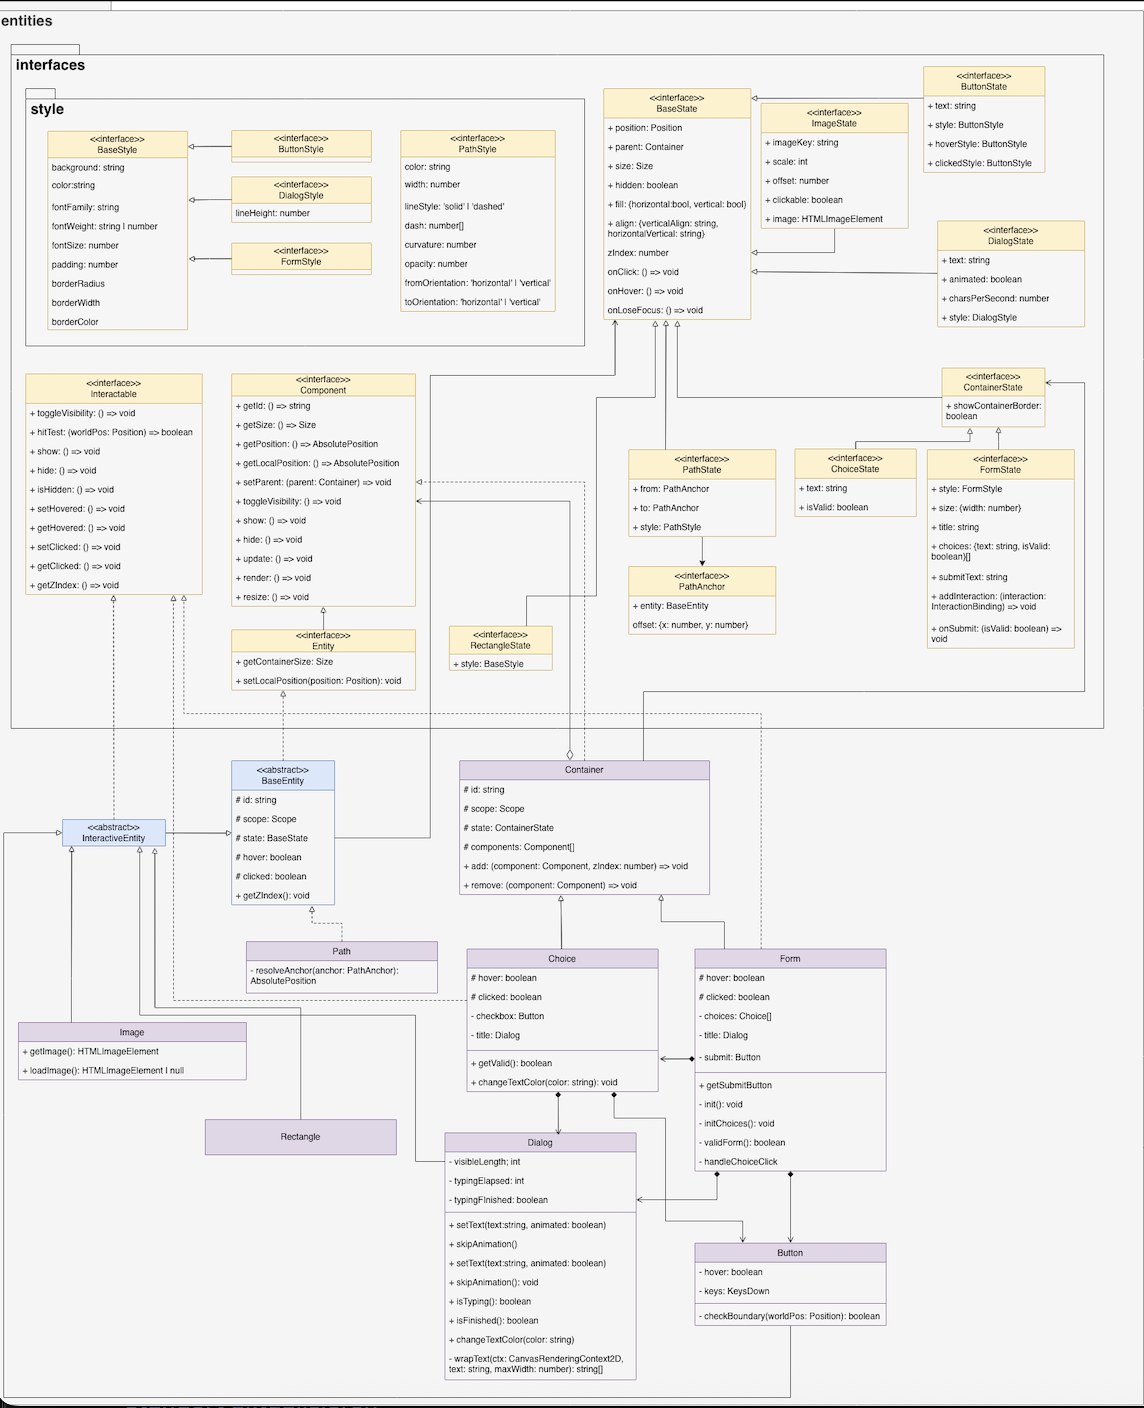
\includegraphics[width=0.85\textwidth]{figures/ClassDiagram_Entities.png}
    \caption{Entity-System und Spezialisierung der generischen Szenentypen}
    \label{fig:engine_entities}
\end{figure}

Die Darstellung erfolgt über ein \textbf{Entity-System}. Jedes grafische Element ist eine Instanz einer \texttt{Entity}-Klasse mit eigenem Lebenszyklus (\texttt{update} und 
\texttt{render}). Beim Abschluss der finalen \texttt{reward}-Szene wird über ein Callback-System die Methode \texttt{updateCompletedStatus} im Backend aufgerufen, 
wodurch der Fortschritt persistent gespeichert und die Navigation zurück zur Roadmap eingeleitet wird.




\subsection{Projektübergreifende Wartungsarbeiten}
Zusätzlich zur Implementierung der neuen Features wurden allgemeine Wartungsarbeiten am Gesamtprojekt durchgeführt. Diese umfassten das Refactoring bestehender Code-Abschnitte 
sowie die Behebung von Fehlern, um die Stabilität und Wartbarkeit des Systems über den Zeitraum des Praxisprojekts hinaus sicherzustellen.